%*******************************************************************************
%*********************************** First Chapter *****************************
%*******************************************************************************

\chapter{Introduction}  %Title of the First Chapter
\label{chapter 1}

%\setlength{\epigraphwidth}{0.3\textwidth}
%\epigraph{}{\textit{}}

According to the C3S Global Temperature Trend Monitor\footnote{This information was obtained from the Copernicus \href{https://apps.climate.copernicus.eu/global-temperature-trend-monitor}{C3S Global Temperature Trend Monitor} in June 2026. The increase in global temperature is estimated from the ERA5 2 meters air temperature.}, the estimated level of global warming reached 1.43 °C above the 1850–1900 baseline in May 2026. Extrapolating the most recent 30-year linear trend would place the 1.5 °C level around 2029, and even with a drastic reduction in greenhouse gas emissions, this threshold is likely to be exceeded \citep{bevacqua_year_2025}. The resulting Climate Change is increasingly affecting natural and human systems across the globe, making adaptation an urgent priority for governments, industries, and communities. In order to shape effective solutions, it is important to recognize that these changes will not manifest themselves uniformly across the world.

As an example, let us consider the Mediterranean region, which is recognized as one of the world's most prominent climate change hotspots. According to the IPCC, over the coming decades the region is expected to experience accelerated warming, more frequent and intense heatwaves, increasing drought and water scarcity, rising sea levels, and heightened wildfire risk \citep{ali_cross-chapter_2022}. Yet, these changes do not translate into a single, uniform impact. 

Firstly, different sectors are vulnerable to different aspects of climate change. In agriculture, the increase in temperatures will require about 10\% to 16\% more water which will be in general less available due to more severe droughts \citep{masia_modelling_2021}. In the transport sector, higher temperatures reduce aircraft take-off performance, with projected decreases of about 11 t in maximum take-off weight for wide-body aircraft by the end of the century \citep{gallardo_assessing_2026}. Coastal transport infrastructure is instead increasingly threatened by sea level rise, with approximately 896 km of Mediterranean roads and railways projected to experience annual coastal flooding under a 3 $^\circ C$ warming scenario \citep{nawarat_coastal_2026}. In the energy sector, residential electricity demand in Southern Europe is projected to increase by around 8\% due to growing cooling needs, while high temperatures simultaneously reduce the transmission capacity of power lines and the efficiency of thermal power plants, increasing stress on electricity systems during heatwaves \citep{dowling_impact_2013}.

Even within the same sector, climate impacts are rarely uniform. Two airports may experience similar increases in air temperature but differ substantially in operational consequences because of runway length, aircraft fleet composition, elevation, or traffic patterns. Likewise, two agricultural areas exposed to comparable warming may face very different risks depending on crop type, irrigation infrastructure, soil characteristics, and water availability. Coastal infrastructures are similarly affected by local topography, shoreline morphology, and existing protection measures. And the complexity extends well beyond the physical impacts of climate change. Adaptation decisions are also shaped by geopolitical dynamics, regulatory frameworks, economic constraints, stakeholder priorities, and the costs and feasibility of different adaptation measures.

The same complexity becomes even more evident when the perspective is reversed, moving to the needs of those responsible for adaptation. Consider, for example, the manager of an airport seeking to develop an effective climate adaptation strategy. The first requirement would be access to reliable local-scale climate projections describing the expected evolution of relevant hazards, such as heatwaves, extreme precipitation, strong winds, or wildfire risk. However, climate information alone would not be sufficient. To support decision-making, these projections should be translated into metrics directly related to the airport's vulnerabilities and operations, such as the frequency with which temperatures are expected to exceed the operational limits of critical infrastructures or affect aircraft performance. At the same time, the inherent uncertainties of climate projections would require appropriate interpretation and expert guidance.
Beyond climate information, the decision-maker would also need to evaluate the technical feasibility, effectiveness, and costs of alternative adaptation measures, balancing investments against the expected reduction in risk.

The outputs of climate research are rarely available at this level of granularity or with the degree of customization required to support this kind of adaptation decisions. Bridging this gap has become one of the major challenges facing the scientific community: transforming climate research into information that can effectively support decision-making at all scales, from supranational institutions to individual citizens. To borrow Bruno Latour's words, this means transforming climate change from a \textit{matter of fact} into a \textit{matter of concern}\footnote{In Latour's terminology, a \textit{matter of fact} refers to scientific knowledge considered as an objective and established fact, whereas a \textit{matter of concern} emphasizes that the same knowledge acquires meaning only when viewed within the broader network of social, political, economic, and ethical issues to which it is connected.}. With this objective, a new field has emerged, bringing together scientific institutions, boundary organizations, consultancy companies, start-ups, and other actors. Since the early 2000s, it has become known as \textbf{\textit{Climate Services}}, highlighting its ultimate goal of putting climate information at the service of society as a whole.

Despite their growing relevance, Climate Services still face significant challenges in establishing themselves as indispensable tools for decision-making. Positioned at the interface between climate science and practice, they must bridge the gap between the complexity of climate information and the needs of decision-makers \citep{jacobs_next_2020}. Climate models generate vast amounts of data describing multiple possible futures, characterized by deep and layered uncertainties, whereas users typically require concise, robust, and actionable information. At the same time, producing information that is simultaneously scientifically credible, salient, and legitimate remains difficult, particularly given the diversity of decision contexts and the evolving needs of users.

Climate Services providers are themselves highly heterogeneous, each contributing complementary expertise. Academic institutions possess the scientific and technical capabilities required to develop and interpret complex climate datasets, but often lack the operational perspective needed to translate scientific knowledge into decision-ready products. Conversely, consultancy companies and other private actors have extensive experience in responding to user needs, but frequently struggle to identify sustainable business models capable of scaling their services beyond highly customized applications. Furthermore, many Climate Services are developed within research or demonstration projects and often fail to evolve into operational, transferable, and sustainable services, highlighting one of the main bottlenecks identified by recent literature: the difficulty of transitioning from successful prototypes to scalable solutions \citep{guentchev_upscaling_2023}. 

The rapid proliferation of services, tools, and platforms further contributes to an increasingly fragmented landscape, making it difficult for users to identify the most appropriate solution for their specific needs. In addition, the strong context dependency of climate information limits the transferability of successful applications across sectors and geographical regions, increasing both the costs and the complexity of service provision. 
%\cite{Jacobs2020NextGeneration}.
Taken together, these challenges configure Climate Services as a typical \textit{valley of death} between climate research and operational decision-making, where scientifically robust knowledge often struggles to become scalable, sustainable, and widely adopted decision-support tools.

% [immagine https://www.the-waves.org/2020/08/06/ai-startups-and-vc-funding-death-valley-to-avoid/]

At the same time, these challenges create opportunities for new approaches capable of bridging the gap between climate science and decision-making. Among them, \textbf{\textit{Artificial Intelligence (AI)}} has rapidly emerged as one of the most disruptive technologies of the last decade. Its recent diffusion has been largely driven by the extraordinary success of transformer-based foundation models\footnote{The widespread adoption of transformer-based foundation models has been driven primarily by the success of conversational AI assistants, including ChatGPT (OpenAI), Claude (Anthropic), Gemini (Google), and similar systems. Their ability to understand natural language, generate coherent responses, and perform a wide variety of reasoning and information-processing tasks has made these models accessible to a broad public, well beyond the research community.}.

Perhaps the clearest impact of AI on everyday activities is the way it is transforming access to information. Rather than searching for documents, browsing multiple web pages, and extracting the relevant content, users can increasingly obtain tailored answers by directly querying AI systems. This paradigm shift has been summarized by the expression \textit{AI is the new UI}, emphasizing the transition from navigating interfaces to interacting with intelligent agents. One of the most visible consequences is the decline in traffic to information websites and specialized online platforms\footnote{Recent evidence suggests that AI assistants are already changing how users access online information. A study reported by \href{https://www.theguardian.com/technology/2025/jul/24/ai-summaries-causing-devastating-drop-in-online-news-audiences-study-finds}{\textit{The Guardian}} describes the substantial decline in traffic experienced by online news websites following the introduction of AI-generated search summaries. Similar effects have also been observed by users for specialized technical websites and online communities, as discussed in a \href{https://www.reddit.com/r/ChatGPT/comments/1gklrkf/not_surprising_but_interesting_to_see_it}{Reddit discussion} reporting traffic statistics from niche domains.}, as the information they provide can increasingly be accessed through AI-powered assistants. Beyond everyday information seeking, specialized domains are also witnessing the emergence of task-specific AI assistants, including systems designed for clinical history-taking and diagnostic dialogue in medicine \citep{tu_towards_2025} and agents capable of autonomously planning and conducting experiments \citep{boiko_autonomous_2023}.

AI, however, extends well beyond conversational agents. It encompasses a broad family of models and algorithms capable of extracting patterns, relationships, and representations from many different forms of data. The same principle underlying chatbots can therefore be applied to information that is not purely textual, including images, audio, financial time series, sensor measurements, and climate model simulations. Regardless of the application domain, the underlying paradigm remains the same: by learning complex representations directly from large datasets, AI systems can infer relationships and generate tailored outputs without relying on explicitly programmed models.

It is therefore unsurprising that Climate Services are increasingly looking at AI as a promising technology to address many of their current challenges. The possibility of transforming raw climate data and scientific research outputs into tailored, decision-oriented knowledge represents one of the most promising opportunities offered by AI. Research institutions are developing AI-based tools to facilitate the exploration and analysis of large climate datasets\footnote{Examples include \href{https://helmholtz.software/software/awi-gpt}{AWI-GPT}, developed by the Alfred Wegener Institute to facilitate the exploration of scientific and climate-related knowledge, and \href{https://ask.copernicus.eu/}{Ask Copernicus}, a conversational interface designed to support the discovery and interpretation of datasets and products from the Copernicus Programme.}, start-ups are building models to estimate the local economic impacts of climate change\footnote{Examples include \href{https://www.eoliann.com/}{Eoliann}, a climate-tech company developing AI models to quantify physical climate risks and estimate their economic impacts at the asset level, supporting risk assessment and adaptation planning for businesses and financial institutions.}, and emerging AI techniques are paving the way for a new generation of high-resolution climate models capable of overcoming some of the limitations of traditional numerical approaches\footnote{Examples include AI-based Earth system models such as \href{https://github.com/NVlabs/FourCastNet}{FourCastNet} (NVIDIA), \href{https://www.nature.com/articles/s41586-023-06185-3}{GraphCast} (Google DeepMind), and \href{https://www.nature.com/articles/s41586-024-07744-y}{Aurora} (Microsoft Research), which demonstrate how AI can produce high-resolution weather and climate predictions with substantially lower computational costs than traditional numerical approaches.}. Nevertheless, this field is still in its early stages. Current developments are characterized by rapid experimentation and a proliferation of potential applications, while robust operational workflows, established best practices, and widely adopted use cases have yet to emerge.

This fragmentation is particularly relevant since, despite their persistent limitations, Climate Services do not operate in an institutional or methodological vacuum. Over time, they have developed a recognizable organization of practices through which climate information is produced and made trustworthy. Research institutions develop and operate climate models; scientific communities evaluate and compare their outputs; standardized datasets and indicators support consistency across applications; and expert knowledge mediates the interpretation of results and their connection to user needs.

The rapid introduction of Artificial Intelligence has the potential to reshape this organization. AI models can change how climate data are produced, they can generate more flexible and context-specific indicators, and provide new interfaces between heterogeneous climate information and its users. At the same time, these systems introduce new sources of uncertainty and failure that are not always captured by established validation practices. Their behaviour may be difficult to interpret, their outputs may depend on training data or model configurations that are not fully accessible, and apparently plausible results may lack scientific grounding or traceable sources.

This thesis investigates how these new capabilities can be integrated into Climate Services without weakening their scientific foundations. It asks how AI reshapes the production, transformation, and communication of climate information, and which standards, evaluation methods, and forms of grounding are required to make its contribution reliable, reproducible, traceable, and useful for decision-making.

The remainder of this chapter provides the foundations needed to position these contributions. The first section establishes an operational framework for Climate Services, understood as the value chain through which climate research outputs are transformed and connected to decision-making contexts. The second introduces the principal AI paradigms and methods employed in the thesis. The final section brings these elements together, situates the individual research contributions within the Climate Services framework, and presents the structure of the dissertation.

%*********************************** First Section - Climate Services *****************************
\section{Climate Services}
\subsection{Definitions and shared principles}

As discussed above, Climate Services emerged from the need to connect climate research more effectively with decision-making. Over time, the term has come to encompass a wide range of activities, actors, and outputs. Definitions proposed by international organizations and research initiatives therefore emphasize different aspects of Climate Services and reflect the evolution of the field (Table~\ref{tab:climate_services_definitions}).

\begingroup
\setlength{\tabcolsep}{4pt}
\renewcommand{\arraystretch}{1.2}
\begin{longtable}{
    >{\raggedright\arraybackslash}p{0.07\textwidth}
    >{\raggedright\arraybackslash}p{0.19\textwidth}
    >{\footnotesize\raggedright\arraybackslash}p{0.48\textwidth}
    >{\footnotesize\raggedright\arraybackslash}p{0.17\textwidth}
}
\caption{Evolution of selected definitions of Climate Services.}
\label{tab:climate_services_definitions} \\
\hline
\textbf{Year} & \textbf{Institution} & \textbf{Definition} & \textbf{Citation} \\
\hline
\endfirsthead

\multicolumn{4}{c}{\tablename~\thetable{} -- continued from previous page} \\
\hline
\textbf{Year} & \textbf{Institution} & \textbf{Definition} & \textbf{Citation} \\
\hline
\endhead

\hline
\multicolumn{4}{r}{\footnotesize Continued on next page} \\
\endfoot

\hline
\endlastfoot

2001 &
U.S. National Research Council &
The timely production and delivery of useful climate data and knowledge to decision makers. &
\citep{national_research_council_climate_2001} \\

2011 &
JPI Climate &
User-driven development and provision of knowledge for understanding the climate, climate change and its impacts, as well as guidance in its use to researchers and decision makers in policy and business. &
\citep{jpi_climate_strategic_2011} \\

2012 &
World Meteorological Organization (WMO) &
Climate information provided in a way that assists decision making by individuals and organizations. Requires appropriate engagement, an effective access mechanism, and responsiveness to user needs. &
\citep{hewitt_global_2012} \\

2014 &
IPCC AR5 &
Climate services are boundary organizations that provide and facilitate knowledge about climate, climate change, and climate impacts for planning, decision-making, and general societal understanding of the climate system. &
\citep{denton_climate-resilient_2014} \\

2015 &
European Commission &
Transformation of climate-related data, together with other relevant information, into customized products such as projections, forecasts, trends, economic analyses, assessments, counseling on best practices, development and evaluation of solutions, and other climate-related services supporting adaptation, mitigation, and disaster risk management. &
\citep{street_european_2015} \\

2016 &
World Meteorological Organization (WMO) &
Climate services develop and provide science-based and user-specific information relating to past, present, and future climate. They connect natural and socio-economic research with practice and transform climate-related data into customized products and services that support decision making across sectors and scales. &
\citep{world_meteorological_organization_climate_2016} \\

2023 &
Climateurope2 &
The provision of climate information, usually in combination with non-climate information and knowledge, in such a way as to assist decision makers. The service component involves a demand-driven approach, stakeholder engagement, effective access mechanisms, and responsiveness to user needs. &
\citep{villwock_literature_2023} \\

\end{longtable}
\endgroup

Together, these definitions show a gradual shift from the timely delivery of climate data towards the provision of customized and contextualized information, often integrating non-climate and socio-economic knowledge. Despite this broadening, they share a stable conceptual core: Climate Services are based on scientific information about past, present, or future climate conditions, they explicitly support decisions by individuals or organizations, and they respond to the needs and circumstances of their intended users. Their service dimension therefore extends beyond making data available to include the mechanisms through which climate information can be accessed, interpreted, and used.

The diversity of actors, sectors, and decision contexts covered by the field helps explain why no universally accepted definition has emerged. A formulation specific enough to describe one implementation may exclude other activities pursuing the same decision-support objective through different processes or outputs. Rather than seeking an exhaustive definition, \citet{hewitt_climate_2021} therefore describe Climate Services concisely as ``the provision of climate information for use in decision-making.'' This formulation is consistent with the shared characteristics identified by \citet{bessembinder_need_2019}: a scientific basis, an orientation towards user needs, and mechanisms that enable information to be delivered and used effectively.

This dissertation adopts that broad understanding rather than proposing an additional definition. Its flexibility accommodates different implementations, but also leaves important analytical distinctions unresolved. In particular, the literature does not always distinguish clearly between data, information, and knowledge; between products and services; or among the overlapping roles of producers, providers, and users \citep{weichselgartner_evolving_2019}. The following subsection clarify these distinctions and integrate them into the operational framework used in this dissertation.

\subsection{From data to decision-relevant knowledge: an operational framework}

The concepts introduced above can be clarified along two complementary dimensions. The first concerns how climate-related content acquires meaning and relevance through the relationship between data, information, and knowledge. The second concerns how that content is made available and connected to decisions through Climate Products and Climate Services. These distinctions provide an analytical vocabulary for the framework developed below.

The Data--Information--Knowledge--Wisdom (DIKW) hierarchy, commonly associated with \citet{ackoff_data_1989}, provides a useful starting point for the first dimension. In its conventional representation, data are progressively transformed into information, knowledge, and ultimately wisdom. However, the boundaries between information and knowledge remain contested \citep{rowley_wisdom_2007}, as does the assumption that these concepts form a universal linear hierarchy \citep{fricke_knowledge_2009}. The DIKW terminology is therefore used here as a heuristic, not as a rigid model of knowledge production.

\textit{Data} consist of recorded observations, measurements, model outputs, or other representations that have not yet been selected and interpreted for a specific purpose. In Climate Services, they may include observations, reanalyses, forecasts, projections, and model simulations, together with non-climate data on exposure, vulnerability, socio-economic conditions, or operational characteristics. Data become \textit{information} when they are selected, processed, combined, or interpreted in relation to a question or context. The same data may therefore produce different information depending on the purpose of the analysis and the needs of its intended users. \textit{Knowledge} emerges when this information is contextualized through expertise, experience, and an understanding of the problem under consideration \citep{rowley_wisdom_2007,weichselgartner_evolving_2019}. Its relevance depends not on the quantity of information provided, but on whether that information can be understood and related to a specific context. \textit{Wisdom} is not further operationalized because it does not perform a distinct function in the framework developed here. Here, we will broadly consider wisdom as the final stage of Climate Services, when the knowledge produced is put in action and integrated in the decision contexts.

The second dimension distinguishes the output through which climate information is communicated from the activities through which it is connected to its use. Conventional product--service distinctions based on tangibility or commercial exchange \citep{baines_state---art_2007} are of limited value in this domain: climate-related outputs are often digital.

In this dissertation, a \textit{Climate Product} is an identifiable output that contains or communicates climate data or information and can be accessed with limited direct involvement from its provider. Examples include datasets, indicators, forecasts, projections, maps, reports, models, and digital platforms. A \textit{Climate Service}, by contrast, comprises the organized activities and interactions through which Climate Products and associated expertise are interpreted, contextualized, or tailored to support a particular decision. This distinction is consistent with \citet{weichselgartner_evolving_2019}: products contain and communicate data or information, whereas services provide the interaction and knowledge exchange that facilitate their use.

Products and services are therefore complementary: a Climate Product may be an essential component of a Climate Service, but its availability alone does not make its information relevant or usable in a particular context. For example, a digital platform may function as a standalone Climate Product or as part of a Climate Service when accompanied by interpretation, user support, or contextualization.



%*********************************** Second Section - Artificial Intelligence *****************************

\section{Artificial Intelligence}

The framework introduced in the previous section describes Climate Services as a set of relationships through which data are transformed into information and connected to decision-relevant knowledge. Artificial Intelligence (AI) is particularly relevant to this process because it can modify both how information is extracted from complex data and how users access, explore, and interpret it. In this sense, AI does not simply introduce new analytical tools: it can reshape the flow of information between scientific content and the users.

AI is a broad field encompassing computational systems designed to perform tasks commonly associated with human intelligence. 
One of its main branches is Machine Learning (ML), which includes algorithms that learn how to perform a task from data rather than relying exclusively on explicitly programmed rules. Although contemporary AI systems can be extremely complex, this underlying principle can be illustrated through one of the earliest and simplest machine-learning models: the Rosenblatt's perceptron \citep{rosenblatt_perceptron_1958}.

The perceptron was developed as a binary classifier capable of assigning an input to one of two possible classes. Given an input vector $x$, its output is defined as

\begin{equation}
    f(x) = \chi\left(\langle w,x\rangle+b\right),
    \label{perceptron}
\end{equation}

where $w$ is a vector of weights, $b$ is a bias term, and $\chi$ is a threshold function. The model combines the input values according to their weights and returns one of the two classes depending on whether the resulting value is above or below a given threshold. During training, the weights and bias are progressively adjusted according to the errors made on a set of examples. The task is therefore not described through a complete sequence of rules: instead, the relationship between inputs and outputs is learned from data.

To handle more complex problems, Artificial Neural Networks (ANNs) extend this principle by connecting many computational units across multiple layers. Each unit computes a weighted combination of its inputs and typically applies a nonlinear activation function. This nonlinearity enables successive layers to construct increasingly abstract internal representations and to capture relationships that cannot be represented by a single linear classifier. A major milestone was reached with the introduction of the back-propagation algorithm, which could be used to train multilayer networks by propagating output errors backwards and adjusting the connection weights accordingly \citep{rumelhart_learning_1986}. Networks containing several intermediate, or hidden, layers form the basis of Deep Learning (DL). DL models have been proven able to learn complex patterns with multiple level of abstraction, achieving outstanding results in may fields such as speech recognition, genomics, and image and video processing   \citep{lecun_deep_2015}. Even if the Rosenblatt's Perceptron is now outdated, most of the recent AI systems are based on DL principles: they combine complex and stratified architectures which are able to learn hidden data patterns learning by examples.

In the context of this thesis, we will focus on the applications of some of such systems. These applications can be distinguished according to the role they play in the transformation of climate data into applicable knowledge, and consequently in the place they can occupy in the Climate Services value chain as depicted above.


\subsection{AI models for weather forecasting and climate simulation}

Weather and climate data describe physical variables distributed across space, altitude, and time, whose meaning depends on the relationships among locations, variables, and successive states. Traditionally, future atmospheric states have been estimated using Numerical Weather Prediction (NWP) models, whereas climate statistics and their response to external forcing have been investigated using General Circulation Models (GCMs) and Earth System Models (ESMs). These models discretize and numerically integrate equations governing atmospheric and oceanic dynamics, thermodynamics, radiation, and interactions among the different components of the Earth system \citep{bauer_quiet_2015}.

In the last few year the scientific community has put a notable effort in developing AI versions of such models. The promise beyond this breakthrough is that these models offer substantial practical advantages. Once trained, AI forecasters and climate emulators can generate forecasts or simulations at a fraction of the computational cost of conventional dynamical models, enabling larger ensembles, denser exploration of forcing scenarios, and rapid sensitivity analyses \citep{van_katwyk_rewiring_2026}. A second major advantage is their adaptability: pretrained and foundation models provide reusable representations that can be fine-tuned for specific regions, variables, spatial resolutions, or downstream applications, while regional emulators can transform coarse global projections into locally relevant climate information \citep{kendon_potential_2025}. 

FourCastNet was among the first global AI systems to demonstrate that neural networks could generate high-resolution medium-range forecasts at a fraction of the computational cost of numerical weather prediction \citep{pathak_fourcastnet_2022}.  It was followed by Pangu-Weather and GraphCast, which showed that such models could match or outperform leading deterministic operational forecasts across many variables and lead times \citep{bi_accurate_2023,lam_learning_2023}. Subsequent developments broadened the methodological scope: NeuralGCM combined a differentiable numerical solver with learned representations of unresolved processes, demonstrating that hybrid physics--AI models can support both medium-range forecasting and stable multi-decadal simulations \citep{kochkov_neural_2024}, whereas GenCast employed a generative diffusion architecture to produce skilful probabilistic forecast ensembles \citep{price_probabilistic_2025}. Recently, ECMWF's fully data-driven AIFS marked the transition of AI forecasting from research prototypes to operational use \citep{moldovan_aifs_2026}, certifing the maturity of AI based weather forecasting models. 

\begin{figure}[H]
    \centering
    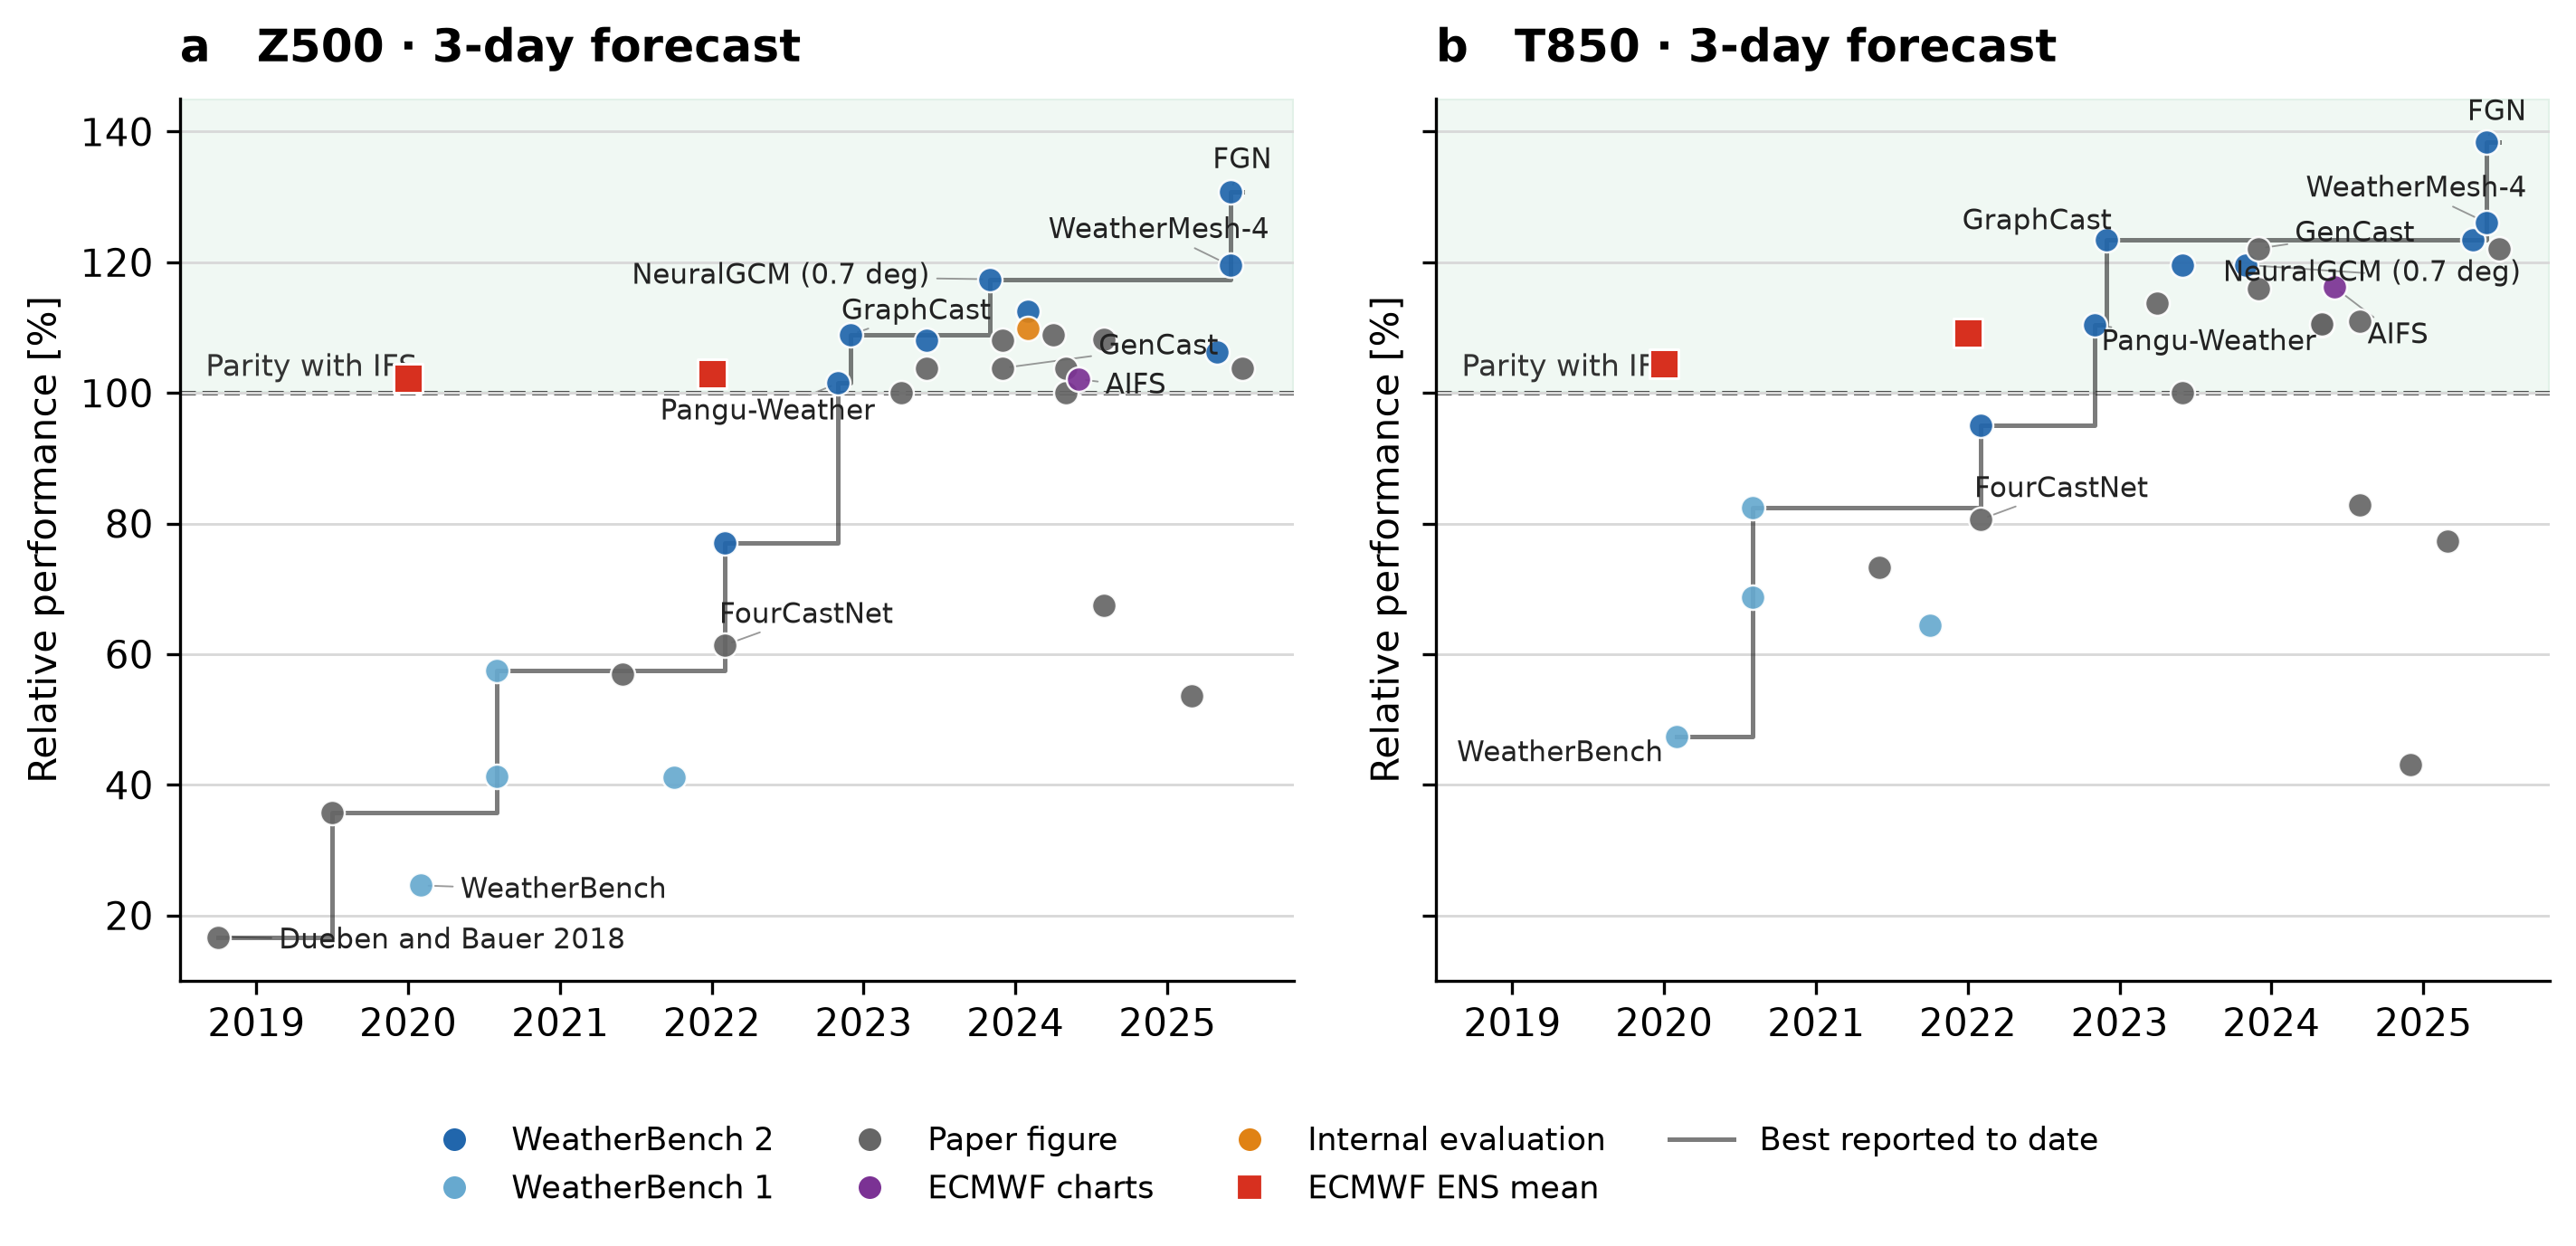
\includegraphics[width=1\linewidth]{Chapter1//figs/ai_weather_progress_relative.png}
    \caption{Evolution of global AI-based weather forecasting performance between 2018 and 2025 for three-day predictions of 500-hPa geopotential (Z500; left) and 850-hPa temperature (T850; right). Performance is expressed relative to the corresponding IFS reference as $100 \times \mathrm{RMSE}_{\mathrm{IFS}}/\mathrm{RMSE}_{\mathrm{model}}$; a value of 100 therefore indicates parity with IFS, while values above 100 indicate lower forecast error. The shaded region identifies models outperforming their IFS reference, and the step line shows the best reported performance up to each date. Colours distinguish the source of the evaluation, while red squares indicate the ECMWF ensemble mean. Because the results originate from heterogeneous evaluation periods, initial conditions, resolutions, and verification protocols, the figure illustrates the overall development of the field rather than providing a strict ranking of individual models. Data adapted from \citet{rasp2024aiweather}.}
    \label{fig:ai_weather_progress}
\end{figure}

AI models, however, are not limited to short- and medium-range weather forecasting. A distinct line of research aims to develop climate emulators capable of producing stable multidecadal simulations under prescribed boundary conditions and forcing scenarios, thereby moving towards capabilities traditionally associated with GCMs and ESMs. The emergence of such models has motivated the AI Model Intercomparison Project (AIMIP), which adapts the model-intercomparison philosophy of AMIP and CMIP to AI-based climate models \citep{henn_aimip_2026}. Initial AIMIP results indicate that these models can reproduce many features of the historical mean climate and atmospheric variability with skill comparable to a conventional numerical model, but also reveal model-dependent underestimation of observed warming trends and divergent responses under out-of-distribution warming scenarios.

Even if the capabilities of these models are already outstanding (Figure \ref{fig:ai_weather_progress}), realizing the potential of these models for Climate Services still requires overcoming both infrastructural and scientific challenges. From an infrastructural perspective, these models depend on specific training and inference methodologies, different requirements for their execution and formats for the input data. From a scientific perspective, their outputs require validation that extends beyond conventional measures of forecast accuracy. Statistical skill must be considered together with physical consistency, multivariate relationships, the representation of extremes, and robustness under conditions that differ from those included in the training data. In concrete, these means that the rapidly evolving and fragmented landscape of AI models for weather forecasting and climate simulation needs to be standardized into frameworks that can make their use reproducible, reliable, and robust.


\subsection{Diagnostic AI models}

Predictive models presented in the section above learn how atmospheric states evolve over time. Prediction, however, is only one way in which AI can operate on weather and climate data. A complementary application is diagnostic: rather than advancing the state of the atmosphere in time, machine learning methods identify coherent structures within observations, reanalyses, and climate simulations and transform them into climate information \citep{schneider_esa-ecmwf_2022}.

An important advantage of this approach is the possibility of constructing diagnostics that are more complex and more closely tailored to a specific scientific or operational purpose. Many conventional climate indices are defined through fixed thresholds, linear combinations, or a small number of variables. Although these indices remain transparent and physically interpretable, they may not fully represent phenomena arising from nonlinear, multivariate, and spatially heterogeneous interactions. Machine learning methods can instead combine multiple atmospheric, oceanic, and surface variables, account for their spatial and temporal dependencies, and learn specific mappings between physical conditions and quantities of interest. This makes it possible to derive data-driven indicators targeted for the most different uses \citep{molina_review_2023}.

The flexibility of diagnostic AI also introduces substantial methodological challenges. Model architectures must be able to represent multivariate spatio-temporal dependencies across different scales while preventing the algorithm from exploiting spurious correlations or dataset-specific features. Validation is particularly challenging because, unlike forecast verification, a unique ground truth may not exist for latent climate regimes or newly learned indicators. Evaluation should therefore combine conventional performance metrics, tests of physical consistency, and interpretability. 

 
\subsection{Large Language Models}

The methods discussed above transform numerical Earth System data into forecasts and climate descriptors. However, producing climate information does not by itself make it accessible, interpretable, or relevant to a particular decision context. A further challenge is to connect numerical outputs with the scientific, technical, and operational knowledge through which they acquire meaning, and to enable users to explore this heterogeneous information according to their specific questions.

Language is central to this process. Scientific findings are communicated through publications and reports, operational procedures are described in technical documentation, and user needs are expressed through questions, discussions, and descriptions of specific problems. Integrating the generalization capabilities of AI with language capabilities is one of the most impacting technological development of the last decades.

An important step in this direction was the development of methods for representing words as numerical vectors. Early neural language models learned both a representation of each word and the probability of observing it within a sequence \citep{bengio_neural_2003}. Later approaches such as Word2Vec made it possible to learn these representations efficiently from large textual collections \citep{mikolov_efficient_2013}. Words appearing in similar linguistic contexts tend to occupy similar positions in the resulting multidimensional space, allowing part of the syntactic and semantic structure of language to be represented in a form that can be processed by machine learning models.

A second major development was the introduction of the Transformer architecture \citep{vaswani_attention_2017}. Its central mechanism, known as \textit{self-attention}, allows the representation of each element of a text to be constructed by considering its relationships with the other elements in the sequence. The meaning assigned to a word can therefore depend on the surrounding context rather than on the word in isolation. Moreover, unlike recurrent architectures, Transformers can process different positions of a sequence in parallel during training. Combined with increasingly large textual datasets and computational resources, this property enabled the training of models with a rapidly growing number of parameters.

Large Language Models (LLMs) are high-capacity neural language models, generally based on the Transformer architecture, trained on extensive and heterogeneous textual corpora. They process text by dividing it into elementary units called \textit{tokens}, which may correspond to entire words, parts of words, punctuation marks, or individual characters. In an autoregressive LLM, the model estimates the probability of the next token on the basis of the preceding sequence. During generation, a token is selected from the predicted probability distribution and appended to the sequence. The updated sequence is then used to predict the following token, and the process is repeated iteratively. 

Following the introduction of the Transformer, the development of LLMs accelerated through a combination of model scaling, post-training, and broader accessibility. GPT-3 demonstrated that increasing model and dataset size could produce strong zero- and few-shot performance, allowing a single pretrained model to address previously unseen tasks from instructions or examples provided directly in its input context \citep{brown_language_2020}. Instruction tuning and reinforcement learning from human feedback subsequently transformed pretrained language models into systems better able to follow user requests, as demonstrated by InstructGPT \citep{ouyang_training_2022}. GPT-4 extended this trajectory through improved performance across academic and professional benchmarks and the integration of textual and visual inputs \citep{openai_gpt-4_2023}, while open-weight model families such as Llama 2 made high-capacity pretrained and dialogue-optimized models more accessible to the broader research community \citep{touvron_llama_2023}. More recently, reasoning-oriented models have combined multi-stage post-training and reinforcement learning to improve performance on tasks requiring extended intermediate reasoning \citep{deepseek-ai_deepseek-r1_2025}. The rapid progression resulting from these developments is illustrated in Figure~\ref{fig:llm_benchmark_progress}.

\begin{figure}[H]
    \centering
    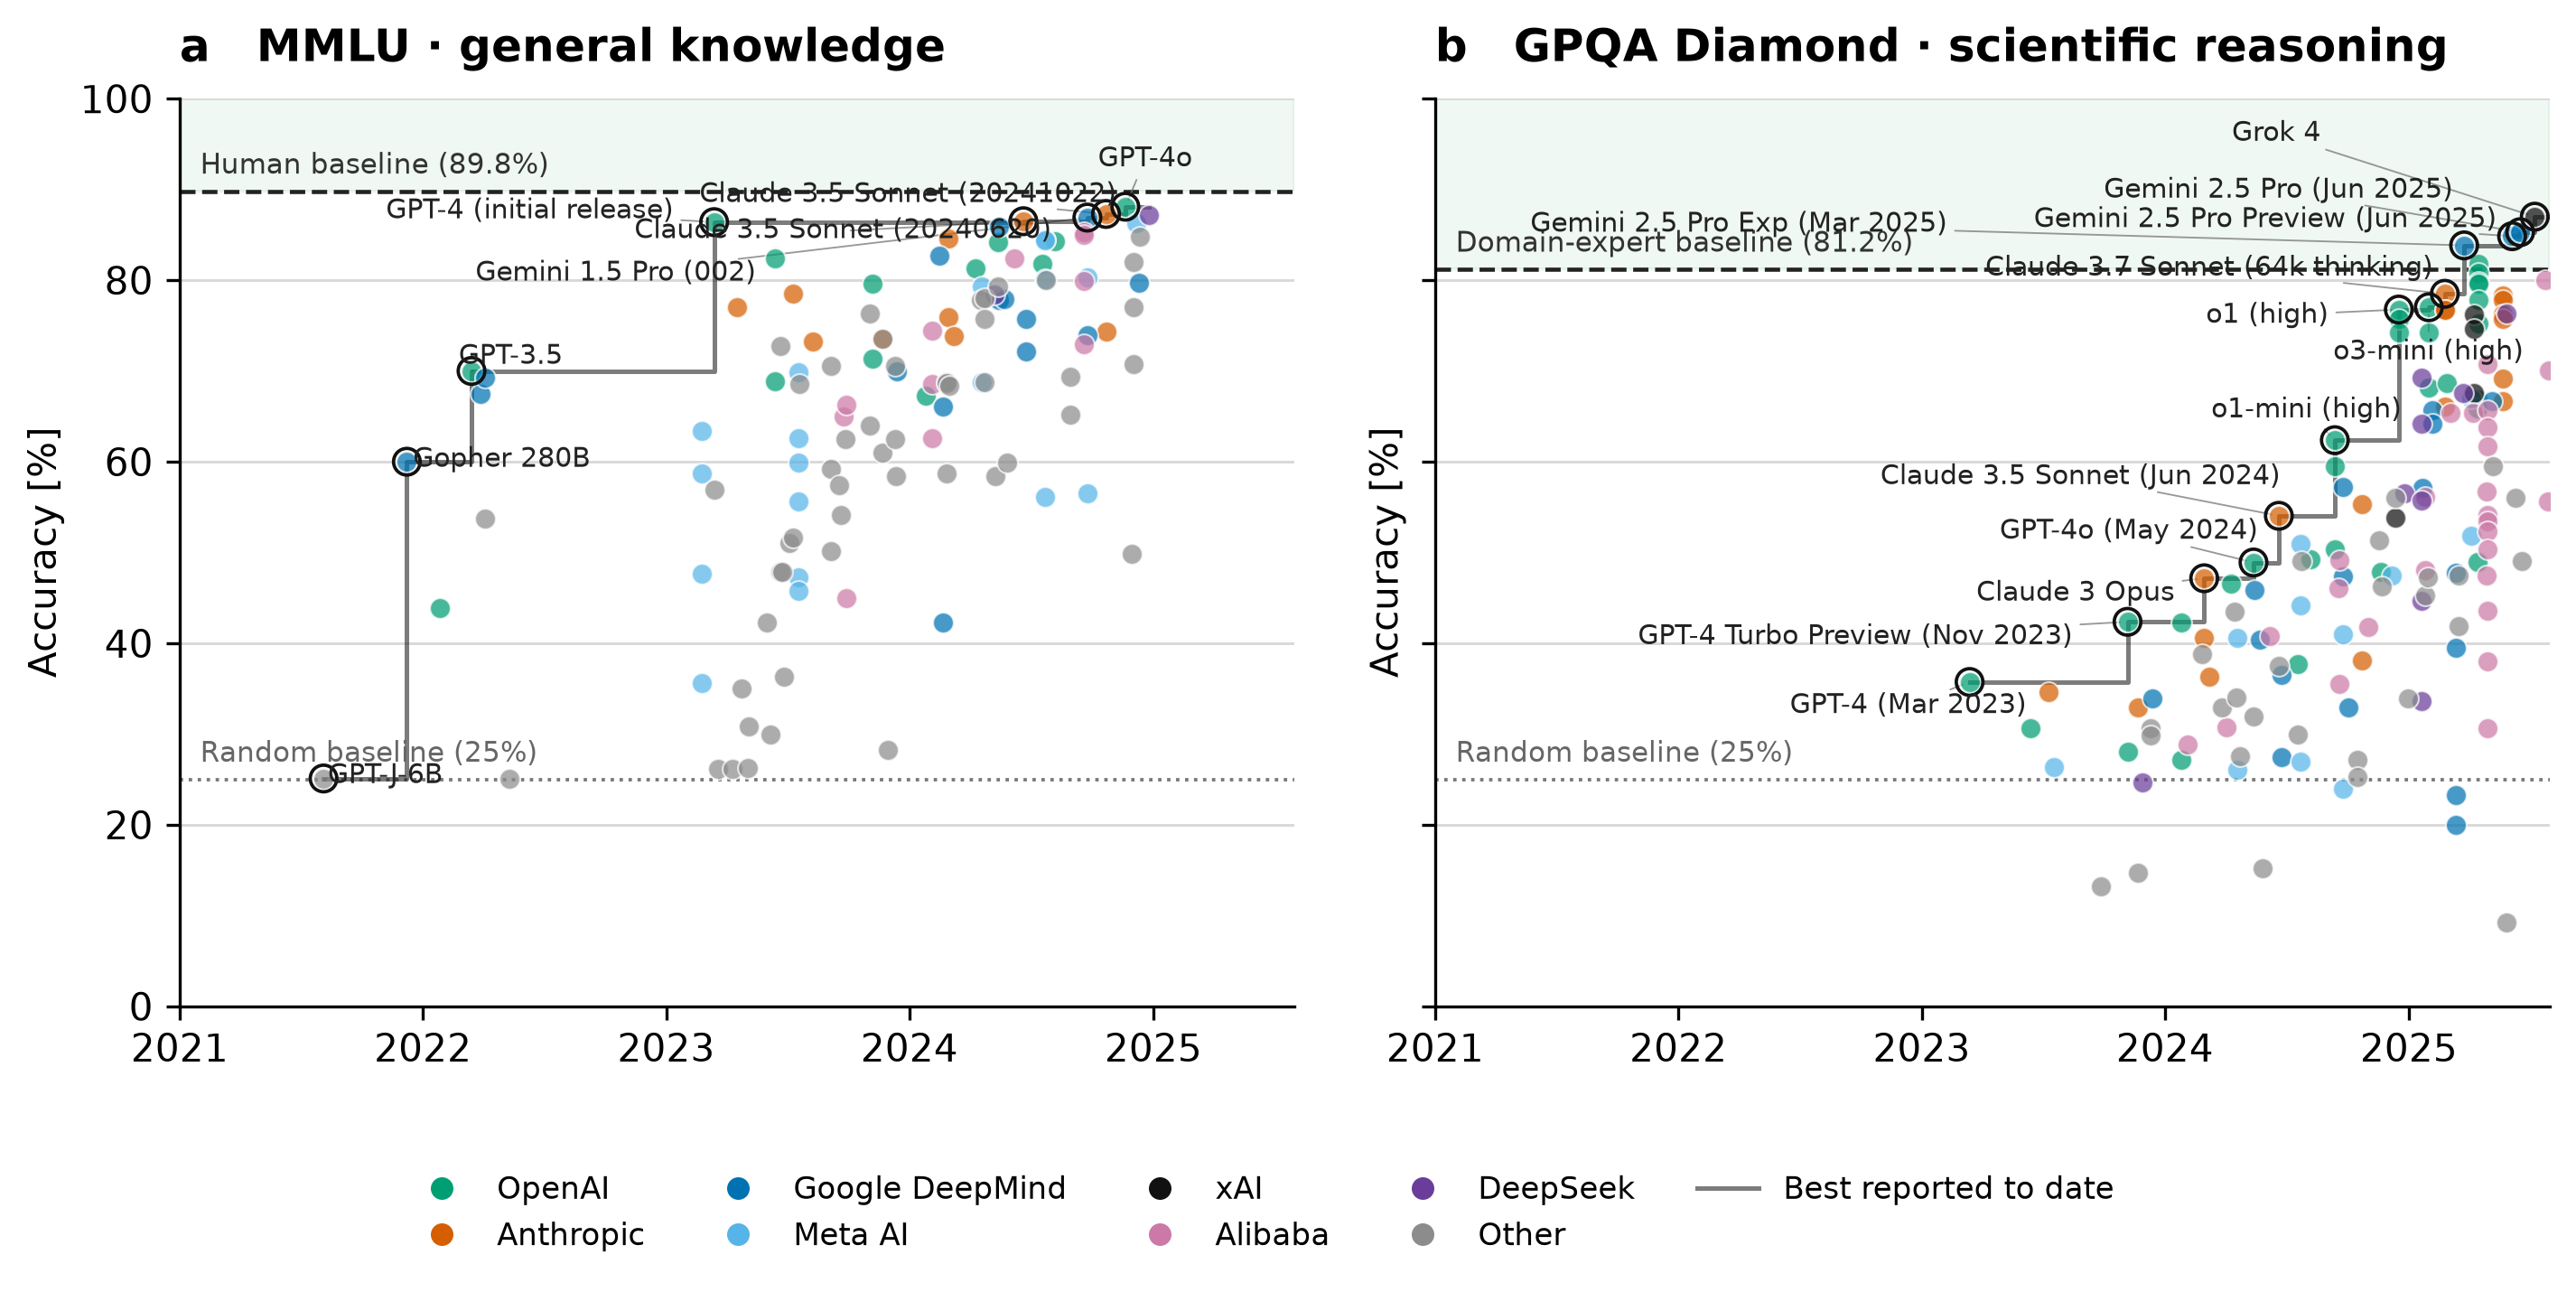
\includegraphics[width=1\linewidth]{Chapter1/figs/llm_benchmark_progress.png}
    \caption{Evolution of Large Language Model performance on MMLU and GPQA Diamond through July 2025. MMLU evaluates broad academic and professional knowledge across 57 subjects \citep{hendrycks2021mmlu}, whereas GPQA Diamond comprises graduate-level questions in biology, chemistry, and physics selected for their difficulty and expert-validated answers \citep{rein2024gpqa}. Each point represents a model evaluation and colours identify the developing organization. Black-outlined markers indicate models that established a new performance frontier, while the step line shows the best reported accuracy available at each date. The dotted line represents random-guessing accuracy (25\%), and the dashed lines show the reported human reference levels: 89.8\% for MMLU \citep{maslej2025aiindex} and 81.2\% for GPQA Diamond \citep{rein2024gpqa}. The shaded regions identify scores above these human references. MMLU results are restricted to five-shot evaluations, while GPQA Diamond values correspond to mean scores reported by the Epoch AI benchmarking framework \citep{epoch2026benchmarking}. Since MMLU results originate from heterogeneous external evaluations that may differ in prompting and implementation details, the figure illustrates the overall progression of benchmark performance rather than providing a strict ranking of individual models.}
\label{fig:llm_benchmark_progress}
\end{figure}

As their scale has increased, LLMs have consequently shown the ability to perform a broad range of tasks through the same linguistic interface, including summarizing documents, extracting relevant information, connecting concepts, and adapting explanations to different questions or audiences \citep{li_fundamental_2024}. The ability to perform different tasks through the same linguistic interface positions LLMs not merely as text generation systems, but as potential interfaces to information. A potential application concerns the fact that the same general-purpose technology can provide meaningful access to the heterogeneous knowledge base underpinning Climate Services. This knowledge is distributed across scientific papers, institutional and technical reports produced for different purposes and audiences, numerical climate datasets, geospatial information, and climate-model outputs. A natural language interface may reduce the technical effort required to formulate a query, access information, and produce tailored knowledge. 

But the versatility and power of LLMs generative capabilities also raises fundamental questions on how their output can be evaluated, both in terms of factual accuracy and epistemic quality for Climate Services purposes.  


%*******************************************************************************
%**************** Third Section - Research framework and thesis outline ********
%*******************************************************************************
\section{Research framework and thesis outline}

The previous sections introduced the operational framework of Climate Services and the main Artificial Intelligence paradigms examined in this thesis. This section brings the two fields together and positions the research contributions along the Climate Services value chain. The central research question is how AI can improve both the production of climate information and its transformation into accessible, specific, and relevant knowledge, and how its outputs should be evaluated to ensure that they remain scientifically reliable. 

As seen in the previous sections, AI is a broad and highly heterogeneous field, encompassing a wide range of concepts, methods, and algorithms. A comprehensive review of its potential applications is therefore beyond the scope of this dissertation. Instead, this thesis adopts a selective approach. It examines a set of representative AI applications positioned at different stages of the Climate Services value chain, from the production of climate data to their transformation into information and decision-relevant knowledge. Rather than attempting to catalogue all possible uses of AI, the thesis investigates the opportunities offered by selected AI paradigms and the methodological requirements needed to integrate them into scientifically robust and operationally useful Climate Services.

Against this background, the following chapters present the research contributions through the methodological frameworks, use cases, and evaluation approaches developed during the research period:

\begin{itemize}

\item Chapter~2 introduces AIUQ, a framework developed in collaboration with the Barcelona Supercomputing Center. AIUQ standardizes the inference workflow of AI-based weather forecasting models, reducing the operational complexity involved in producing large ensembles of simulations with heterogeneous models. It also introduces an evaluation framework for testing their out-of-sample behavior and assessing their ability to generalize across configurations and climatic conditions that differ from those encountered during training. This chapter addresses the first step of the Climate Services value chain: the reliable, robust, and reproducible production of climate data through AI.

\item Chapter~3 moves from prediction to diagnosis by introducing a machine-learning framework for deriving objective, data-driven definitions of meteorological seasons from reanalysis data and applying them consistently to climate-model projections. The framework is applied to the Indian subcontinent, where seasonality has major societal and economic implications because of the monsoon and where the extensive scientific knowledge available provides a strong basis for validating the proposed approach. This chapter addresses the second step of the Climate Services value chain: the transformation of climate data into information through AI, while examining the practical advantages of data-driven algorithms over deterministic definitions.

\item Chapter~4 introduces the contribution of Large Language Models to Climate Services by addressing a first fundamental evaluation question: to what extent do LLMs encode reliable climate information in their parametric knowledge? To answer this question, a practical benchmark for assessing the climate knowledge of different LLMs was developed at the Alfred Wegener Institute and applied to a selection of open-source and proprietary models. Within the Climate Services value chain, this chapter examines the capacity of LLMs to retrieve, connect, and communicate information as a basis for knowledge creation.

\item Chapter~5 addresses a second fundamental question: how can the epistemic quality of LLM outputs be evaluated in the context of Climate Services? The chapter introduces a framework that assesses answers to climate-related questions along four dimensions: relevance, actionability, credibility, and uncertainty communication. The framework is then applied to four LLM-based systems implementing different augmentation strategies and interacting with different sources of climate knowledge: textual information retrieval, operations on numerical climate data, and combinations of the two. This chapter addresses the transition from information to knowledge by examining how LLMs can contextualize heterogeneous climate content while preserving the qualities required for its use in Climate Services.

\end{itemize}

Figure~\ref{fig:research_framework} summarizes the relationship between the operational framework of Climate Services and the contributions of the thesis.

\begin{figure}[H]
\centering
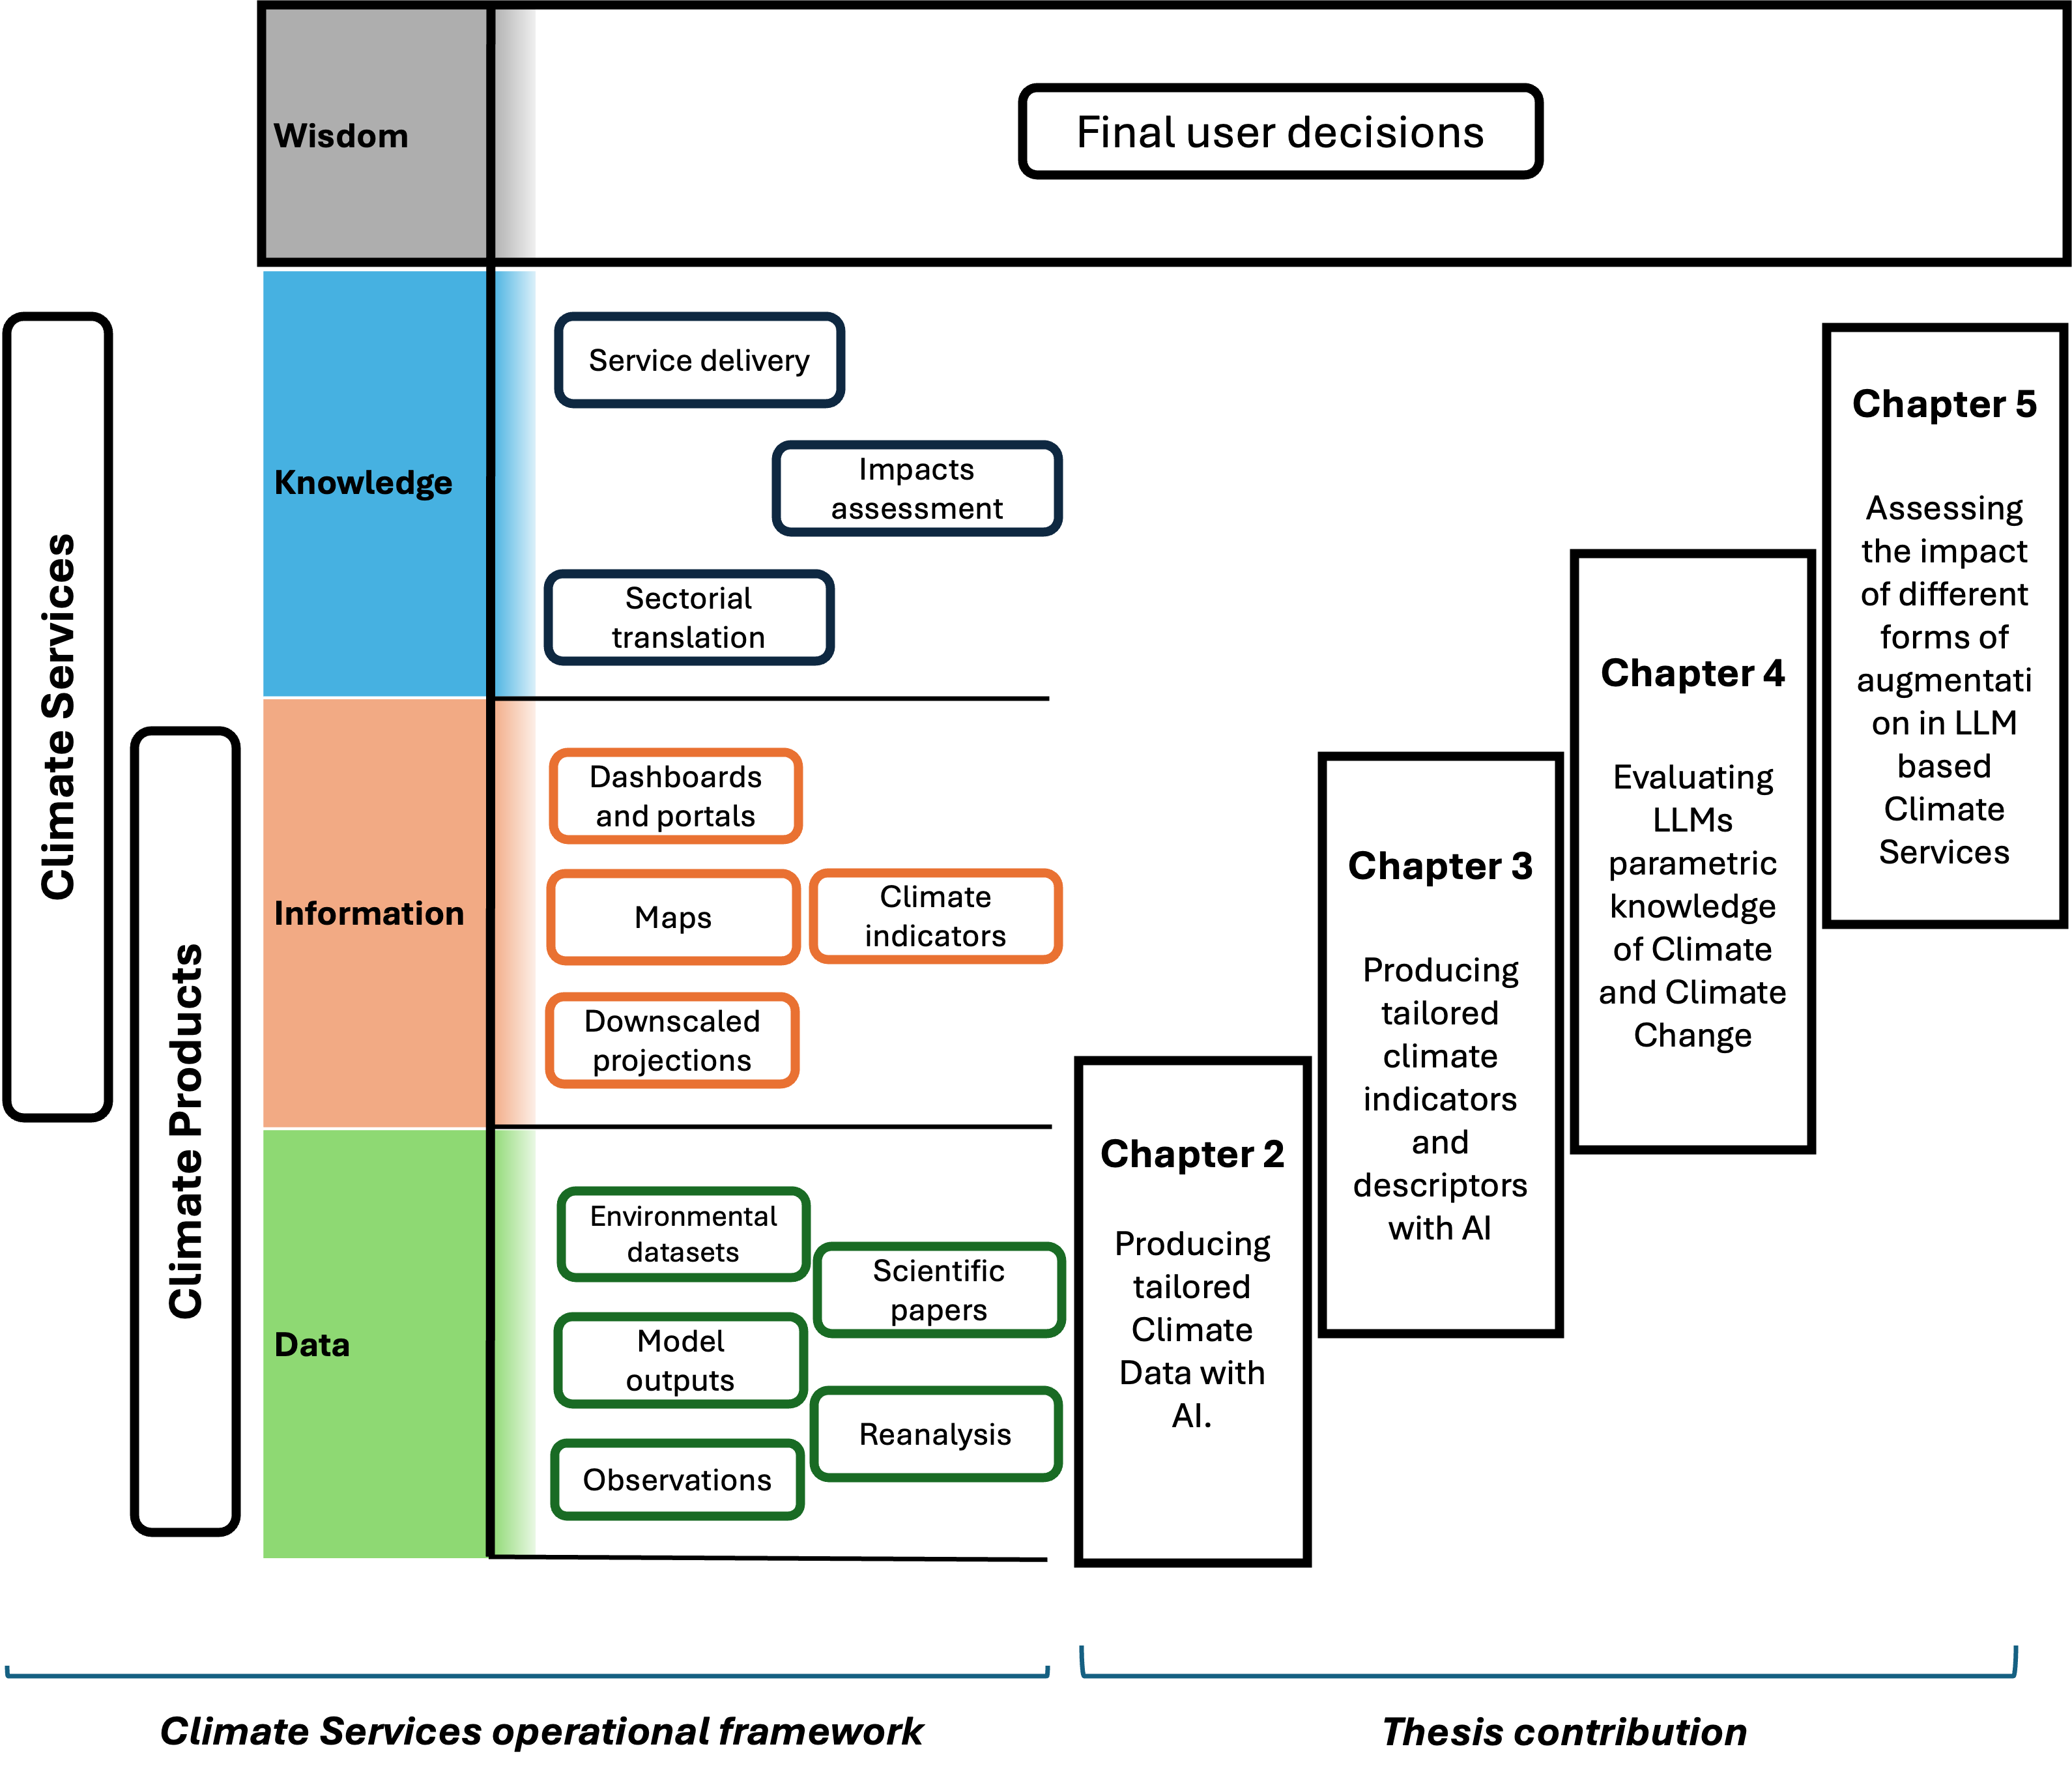
\includegraphics[width=\linewidth]{Chapter1/figs/framework.png}
\caption{Conceptual framework linking the operational structure of Climate Services to the contributions of this thesis. The left-hand panel represents the progression from heterogeneous climate data to information, knowledge, and ultimately decision-relevant wisdom, while distinguishing Climate Products from the broader Climate Services through which these products are interpreted and connected to their use. The right-hand panel positions Chapters~2--5 within this progression.}
\label{fig:research_framework}
\end{figure}

